\documentclass[a4paper,11pt]{article} % screen setting

\usepackage[a4paper]{geometry}
\geometry{verbose,tmargin=1.5cm,bmargin=1.5cm,lmargin=1.5cm,rmargin=1.5cm}

\setlength{\parskip}{\smallskipamount}
\setlength{\parindent}{0pt}

%\usepackage{fontspec}
\usepackage[libertine]{newtxmath}
\usepackage[no-math]{fontspec}
\setmainfont{Linux Libertine O}
\setmonofont{DejaVu Sans Mono}

\usepackage{hyperref}
\usepackage{url}
\usepackage{xcolor}

% DARKMODE
%\pagecolor[rgb]{0,0,0} %black
%\color[rgb]{0.8,0.8,0.8} %grey

\usepackage{amsmath}
\usepackage{amssymb}

\usepackage{graphicx}
\usepackage{float}

\usepackage{minted}

\newminted{dart}{breaklines,fontsize=\footnotesize}
\newminted{bash}{breaklines,fontsize=\footnotesize}
\newminted{text}{breaklines,fontsize=\footnotesize}

\newcommand{\txtinline}[1]{\mintinline[breaklines,fontsize=\footnotesize]{text}{#1}}
\newcommand{\dartinline}[1]{\mintinline[breaklines,fontsize=\footnotesize]{python}{#1}}

\newmintedfile[pythonfile]{python}{breaklines,fontsize=\footnotesize}

\definecolor{mintedbg}{rgb}{0.90,0.90,0.90}
\usepackage{mdframed}
\BeforeBeginEnvironment{minted}{
    \begin{mdframed}[backgroundcolor=mintedbg,%
        topline=false,bottomline=false,%
        leftline=false,rightline=false]
}
\AfterEndEnvironment{minted}{\end{mdframed}}


%\usepackage{setspace}
%\onehalfspacing

\usepackage{appendix}

\newcommand{\highlighteq}[1]{\colorbox{blue!25}{$\displaystyle#1$}}
\newcommand{\highlight}[1]{\colorbox{red!25}{#1}}

\newcounter{soal}[section]
\newenvironment{soal}[1][]{\refstepcounter{soal}\par\medskip
   \noindent \textbf{Soal~\thesoal. #1} \rmfamily}{\medskip}

\begin{document}


\title{Quiz Dart dan Flutter 2}
\author{}
\date{}
\maketitle


Tugas ini adalah pengganti untuk UAS.

Buat aplikasi Flutter untuk menampilkan plot sederhana dari:
\begin{itemize}
\item Dekomposisi sinyal periodik dengan deret Fourier: misalnya sinyal kotak, sinyal
segitiga, dan sebagainya \footnote{\url{https://en.wikipedia.org/wiki/Fourier_series}}, dan
\item Kurva Lissajous \footnote{\url{https://en.wikipedia.org/wiki/Lissajous_curve}}
\end{itemize}

Untuk membuat plot tersebut, kita dapat menggunakan pustaka \txtinline{charts_flutter}
yang dapat dilihat pada {\footnotesize\url{https://pub.dev/packages/charts_flutter}}.

Contoh program dapat dilihat pada kode berikut ini. Karena dua plot yang akan kita buat
berdasarkan pada fungsi sinusoidal, kita akan membuat plot fungsi sin.
\begin{dartcode}
import 'package:charts_flutter/flutter.dart' as charts;
import 'package:flutter/material.dart';
import 'dart:math' as math;
  
void main() => runApp(MyApp());

class MyApp extends StatelessWidget {
  @override
  Widget build(BuildContext context) {
    return MaterialApp(
      title: 'Quiz 2 Flutter',
      theme: ThemeData(
        primarySwatch: Colors.blue,
      ),
      home: Scaffold(
        appBar: AppBar(
          title: Text('Plot Fungsi'),
        ),
        backgroundColor: Colors.white,
        body: Container(
          width: 500,
          height: 400,
          child: SimpleLineChart.withSampleData(),
        ),
      ),
    );
  }
}

class Point {
  final double x;
  final double y;
  Point(this.x, this.y);
}

class SimpleLineChart extends StatelessWidget {
  final List<charts.Series> seriesList;
  final bool animate;

  SimpleLineChart(this.seriesList, {this.animate});

  /// Creates a [LineChart] with sample data and no transition.
  factory SimpleLineChart.withSampleData() {
    return new SimpleLineChart(
      _createSampleData(),
      // Disable animations for image tests.
      animate: false,
    );
  }

  @override
  Widget build(BuildContext context) {
    return new charts.LineChart(seriesList, animate: animate);
  }

  static List<charts.Series<Point, double>> _createSampleData() {
    List<Point> data = List<Point>();
    const double xi = 0.0;
    const double xf = 1.0;
    const double L = xf - xi;
    const int Ndata = 100;
    double deltax = (xf - xi)/(Ndata-1);
    for(int i = 0; i < Ndata; i++) {
      double x = xi + i*deltax;
      double y = math.sin(2*math.pi*x/L);
      data.add(Point(x,y));
      print('x = $x, y = $y'); // Opsional, untuk melihat hasil ke terminal
    }
    return [
      new charts.Series<Point, double>(
        id: 'ExamplePlot',
        colorFn: (_, __) => charts.MaterialPalette.blue.shadeDefault,
        domainFn: (Point p, _) => p.x,
        measureFn: (Point p, _) => p.y,
        data: data,
      )
    ];
  }
}
\end{dartcode}

Contoh tampilah program:

{\center
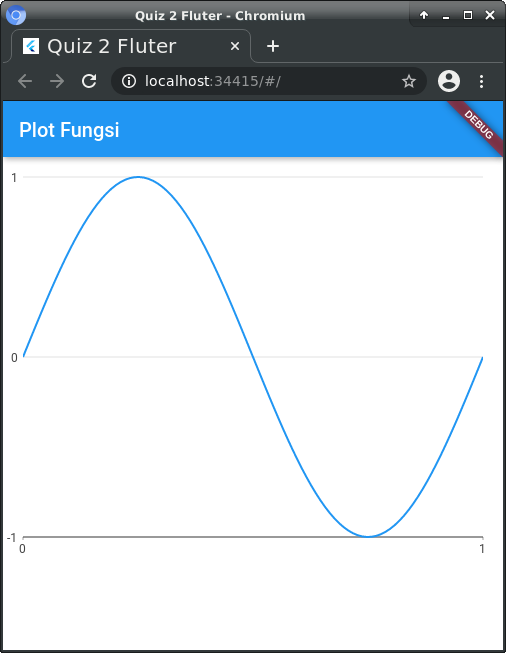
\includegraphics[scale=0.5]{images/PlotSinus.png}
\par}

Spesifikasi minimal aplikasi:
\begin{itemize}
\item Mampu menampikan plot fungsi periodik dengan deret Fourier dan kurva Lissajous
pada halaman yang berbeda, dapat menggunakan menu untuk navigasi atau teknik lain.
\item Sertakan juga halaman developer info yang sudah dibuat pada Quiz 1.
\end{itemize}

Penambahan fitur lain seperti input parameter tidak diwajibkan, namun jika ada
akan mendapat poin tambahan.

Tugas dikumpulkan dalam satu folder yang di-zip dan berisi:
\begin{itemize}
\item Penjelasan singkat dalam file PDF mengenai persamaan matematik dan
kode yang digunakan beserta screenshoot
program (bukan screenshoot kode)
\item File kode Dart yang digunakan (hanya file dengan ekstensi \txtinline{.dart} saja) beserta
file asset yang diperlukan (misalnya untuk gambar).
\end{itemize}

\bibliographystyle{unsrt}
\bibliography{BIBLIO}

\end{document}
